\chapter{Introduction}
\label{chap:intro}

%%%%%%%%%%%%%%%%%%%%%%%%%%%%%%%%%%%%%%%%%%%%%%%%%%%%%%%%%%%%%%%%%%%%%%%%%%%%%%%
\section{Motivation}
\label{sec:chap1-motivation}

%Intro paragraph\\
%-talk about the increasingly important role of simulation in nuclear?\\
%-challenges for today's nuclear fleet which simulation is well-poised to tackle\\
%-segue into talk about nuclear reactor / neutron physics paragraph\\
%-based on empirical models\\
%-need to account for angular dependence of neutron flux (e.g. "transport" methods)\\

Numerical simulation has long played an important role in nuclear reactor physics and engineering. The nuclear industry relies on computational modeling of the neutron physics in reactors to predict core reactivity, power distributions, fuel depletion, and transient behavior to ensure the safety and reliability of the current fleet of Light Water Reactors (LWRs). Predictive simulations are necessary to evaluate innovations which seek to improve reactor safety and fuel cycle economics, such as reduced safety margin uncertainties, accident-tolerant fuels, and extended cycle lengths. In addition, simulation is used to assess the technical competencies of advanced reactor technologies such as Small Modular Reactors (SMRs), Sodium Fast Reactors (SFRs), Molten Salt Reactors (MSRs), High Temperature Gas Reactors (HTGRs), among other proposed designs. 

Many Generation III+ reactors, such as the Westinghouse AP1000\texttrademark \ac{PWR}, optimize performance with complicated core designs. A variety of reactivity control mechanisms -- including partially-inserted control rods, ``grey'' control poisons, \ac{IFBA}, soluble boron, etc. -- along with axial enrichment zoning are used to improve performance metrics such as power peaking factors. The reactor analysis methods in widespread use today assume a ``smoothly'' varying flux distribution, and are not well-suited to model highly localized flux gradients which result from these complex core configurations. New high-fidelity simulation tools are needed to accurately capture neutron physics in advanced reactor designs.

The development and deployment of neutron physics simulations is governed by tradeoffs between accuracy and speed. High-fidelity simulations are accurate and flexible since they make few approximations, but they require significant computational time and resources. On the other hand, the assumptions and approximations made by low-fidelity methods enable optimizations which greatly improve the time-to-solution. However, low-fidelity models are designed for specific applications and lose their predictive power when employed in settings outside of the scope for which they were intended. As a result, it is common to employ a mix of high- and low-fidelity tools for reactor analysis -- for example, high-fidelity tools are frequently used to inform and benchmark low-fidelity models for use within a narrow envelope of design paramters. This thesis develops a new approach within the same vein by employing continuous energy Monte Carlo simulations to generate accurate multi-group cross sections for computationally efficient fine mesh multi-group methods.


%%%%%%%%%%%%%%%%%%%%%%%%%%%%%%%%%%%%%%%%%%%%%%%%%%%%%%%%%%%%%%%%%%%%%%%%%%%%%%%
\section{Background}
\label{sec:chap1-background}

A key trend in recent years has been the steady progress towards whole-core neutron transport-based reactor analysis tools. The standard methods used for reactor analysis today continue to be based on diffusion theory, which enables orders of magnitude computational performance improvements with respect to transport methods. Diffusion-based methods coupled with accurately modeled cross section data have proven to be sufficiently accurate for software tools used by reactor analysts, designers and regulators in industry and academia. However, these techniques rely on a number of assumptions and approximations which are not valid for all reactor types. For example, some Generation IV reactor design concepts are significantly more challenging to model than \ac{LWR}s due to the high degree of spectral coupling between geometrically disparate zones within the core. Although the computational requirements for whole-core transport-based simulations have precluded their widespread deployment, the continuing growth of cheap parallel processing power has made the prospects for such tools increasingly feasible.

%Transport-based methods would enable more accurate core power distributions to be calculated without the approximations needed for today’s tools based upon diffusion theory.

\ac{MC} particle transport methods are often looked to as the ``gold standard'' for the future of nuclear reactor core depletion calculations. Monte Carlo methods are by their very nature reactor agnostic in that they permit an accurate treatment of the core geometry and spectral coupling. Another appealing characteristic of \ac{MC} methods is their ability to effectively use continuous energy cross sections with up to tens of thousands of energy points. An accurate treatment of evaluated cross section data permits high-fidelity core spectral calculations. Although new scalable parallel algorithms have
enabled codes to achieve excellent scaling on 100,000s of cores, production tools for industrial applications remain out of reach for the foreseeable future.

The primary reason for this is that the inverse square root convergence rate inherent to \ac{MC} makes it computationally intractable to realize an acceptably low uncertainty for each tally of interest except on large supercomputers. Furthermore, whole-core Monte Carlo calculations require many terabytes of memory to store the tallied quantities, which is inaccessible except on the world's largest computing machines. Finally, the accurate energy treatment largely renders \ac{MC} methods inefficient for modern computational hardware. The stochastic treatment of the nonlinear neutron energy characterization is challenging to vectorize and results in highly disjoint memory accesses to cross section data with minimal cache reuse. 

An attractive alternative to MC are deterministic methods -- such as Discrete Ordinates (SN), Simplified PN (SPN), and the Method of Characteristics (MOC). Deterministic methods do not make use of continuous energy cross section data and instead discretize the energy domain through the multi-group energy approximation. The multi-group approximation considerably reduces the necessary dataset footprint for simulation. In addition, the multi-group approximation enables deterministic methods to be more readily formulated in such a way as to permit greater vectorization and cache reuse than \ac{MC}. However, the approximation requires an \textit{a priori} estimate of the neutron flux to compute the multi-group cross sections in each region. These cross sections are then used to solve for the flux distribution throughout the core. Many different engineering approximations have been developed to counter this issue for LWRs. For reactors with a greater degree of spectral coupling, however, these approximations are not valid, resulting in ever larger datasets for the cross section generation process. As a result, a new approach for reactor agnostic multi-group cross section generation is needed to make multi-group neutron transport methods a viable option for future reactor analysis tools.

%Deterministic transport methods pose a number of advantages to \ac{MC} from a computational perspective, which seems likely to make these methods more viable in the near to intermediate term. However, deterministic methods almost universally discretize the energy domain in a few to hundreds of energy groups. This approximation requires energy condensed \ac{MGXS} in each geometric region to preserve reaction rates. Accurate \emph{reactor agnostic} multi-group cross section generation is needed to enable deterministic transport-based methods to be as accurate and flexible as Monte Carlo in whole-core calculations.

This thesis investigates the potential use of Monte Carlo methods to generate \ac{MGXS} for next-generation whole-core deterministic reactor analyis. Monte Carlo presents a natural approach to replace engineering prescriptions to approximate the flux with a stochastic approximation of the exact flux. The advantage of a \ac{MC}-based approach is that all of the relevant physics modeled in \ac{MC} may be directly embedded into \ac{MGXS}. This improvement in accuracy comes at the computational expense of converging group constant tallies to acceptably low uncertainties. \ac{MC} methods have increasingly been used to generate few group constants for coarse mesh diffusion, most notably by the Serpent \ac{MC} code~\cite{serpent2013manual}. However, there exist few rigorous and comprehensive analyses of \ac{MGXS} generation from \ac{MGXS} for heterogeneous fine-mesh transport.

\begin{emphbox}
\textbf{The high-level vision underlying this thesis is the desire to obtain Monte Carlo-quality solutions with computationally efficient deterministic neutron transport methods.}
\end{emphbox}

next paragraph: multi-level framework
-intro MGXS
-need the flux to compute MGXS
-black magic ``crux'' of deterministic methods
-talk about decoupling of energy treatment from spatial treatment
  -successively try to embed physics effects from high-fi methods into low-fi methods
  -energy self-shielding effects first, then spatial self-shielding effects
-wish to reduce the number of stages in order to eliminate sources of approx. error and make methods more reactor agnostic or generalizable or predictive

final paragraph: MC 4 MGXS
-motivate \ac{MC} for \ac{MGXS}
-has already been done for some applications
  -esp. coarse mesh diffusion
-must accelerate it in way not possible for conventional \ac{MC}
-efforts to date still retain multi-level approach
  -new methods to consider how to eliminate the levels altogether

\begin{emphbox}
\textbf{This thesis evaluates Monte Carlo-based methods to generate \ac{MGXS} for fine mesh neutron transport codes.}
\end{emphbox}

\begin{figure}
\centering
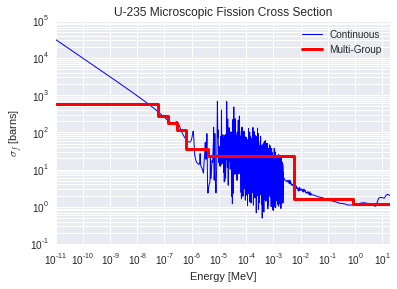
\includegraphics[width=0.9\linewidth]{figures/intro/u235-ce-mg-xs}
\caption[U-235 continuous energy and multi-group fission cross section]{U-235 continuous energy and multi-group fission cross section.}
\label{fig:chap1-multi-level-flow-chart}
\end{figure}

\begin{figure}
\centering
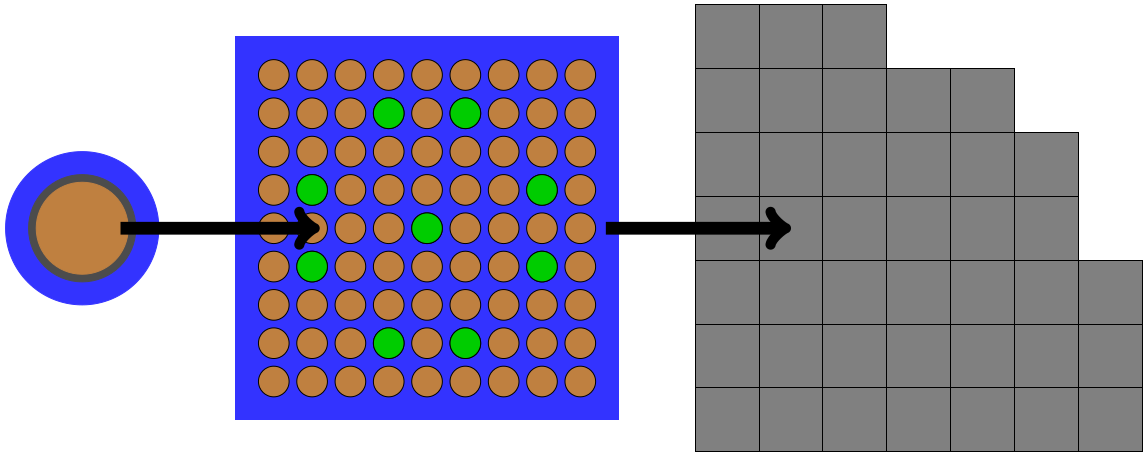
\includegraphics[width=0.9\linewidth]{figures/intro/multi-step-flow-chart}
\caption[Multi-level approach to reactor analysis]{Current multi-level framework for reactor analysis.}
\label{fig:chap1-multi-level-flow-chart}
\end{figure}


%%%%%%%%%%%%%%%%%%%%%%%%%%%%%%%%%%%%%%%%%%%%%%%%%%%%%%%%%%%%%%%%%%%%%%%%%%%%%%%
\section{Thesis Objectives}
\label{sec:chap1-objectives}

%Third paragraph\\
%-mention MG would be the reference soln anyway
%-replace deterministic approximation 
%-Existing codes/techniques may not be adequate for whole-core transport\\

-split up paragraphs according to two high-level themes
-itemize objectives with bullet points

The subject matter of this thesis can be organized along two main themes. First, the efficacy of \ac{MGXS} generation with \ac{MC} for fine-mesh transport calculations is rigorously assessed. Some of the approximations made by \ac{MC}-based \ac{MGXS} generation are quantified, including the energy- and spatial-dependence of condensed \ac{MGXS}. An in-depth analysis of systematic bias resulting from constant-in-angle \ac{MGXS} is presented, along with a scheme based on \ac{SPH} factors to compensate for this loss in accuracy. The second theme of this thesis is focused on a new methodology to simultaneously capture local and global spatial self-shielding effects in \ac{MGXS} for whole-core calcuations. This scheme applies statistical clustering to accelerate convergence rate of \ac{MGXS} tallied on high-fidelity spatial meshes in Monte Carlo. The latent variable model which inspires this new scheme is discussed. A series of increasingly complex case studies empirically compare the accuracy and convergence rate of the scheme with traditional \ac{MC}-based MGXS generation.


%%%%%%%%%%%%%%%%%%%%%%%%%%%%%%%%%%%%%%%%%%%%%%%%%%%%%%%%%%%%%%%%%%%%%%%%%%%%%%%
\section{Thesis Outline}
\label{sec:chap1-outline}

-mention that thesis is broken into three main parts
-break into two paragraphs for each part

Chapter~\ref{chap:intro} motivates the need for new \ac{MGXS} generation techniques with an overview of trends in \ac{HPC} and whole-core transport methods. Chapter~\ref{chap:mgxs} reviews the multi-group cross section approximation, and highlights past efforts to use \ac{MC} to generate \ac{MGXS}. The simulation codes utilized in this thesis are discussed in Chapter~\ref{chap:workflow}, including OpenMC, OpenMOC and OpenCG. The impact of \ac{MGXS} approxmation error is quantified in heterogeneous geometries in Chapter~\ref{chap:biases}. Chapter~\ref{chap:sph} presents an algorithmic approach to address systematic biases resulting from constant-in-angle \ac{MGXS}. A latent variable model for spatial-self shielding effects on \ac{MGXS} is outlined Chapter~\ref{chap:methods}, along with a data pipeline for unsupervised clustering to accelerate the \ac{MGXS} convergence rate. Chapter~\ref{chap:results} evaluates the impact of clustered \ac{MGXS} on the accuracy and convergence rate. Finally, Chapter~\ref{chap:conclusions} summarizes the progress made in this thesis to chart a path forward for \ac{MC}-based \ac{MGXS} generation for whole-core deterministic transport methods.

%\begin{figure}
%\begin{subfigure}{\textwidth}
%  \centering
%  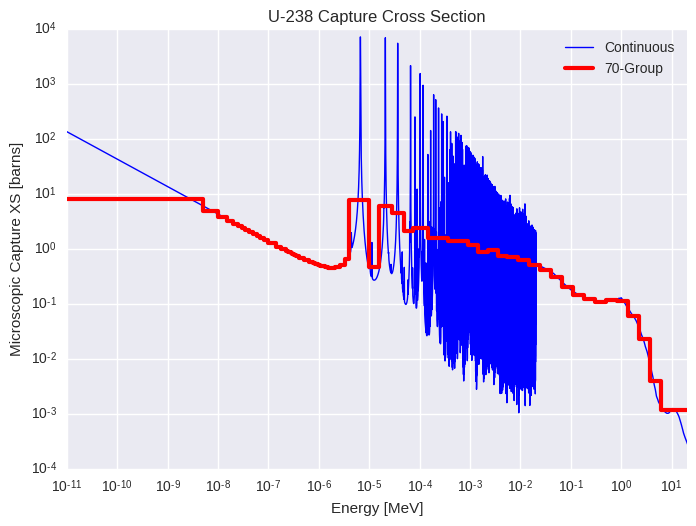
\includegraphics[width=0.9\linewidth]{figures/intro/u238-capture-70}
%  \caption{}
%\end{subfigure}
%\begin{subfigure}{\textwidth}
%  \centering
%  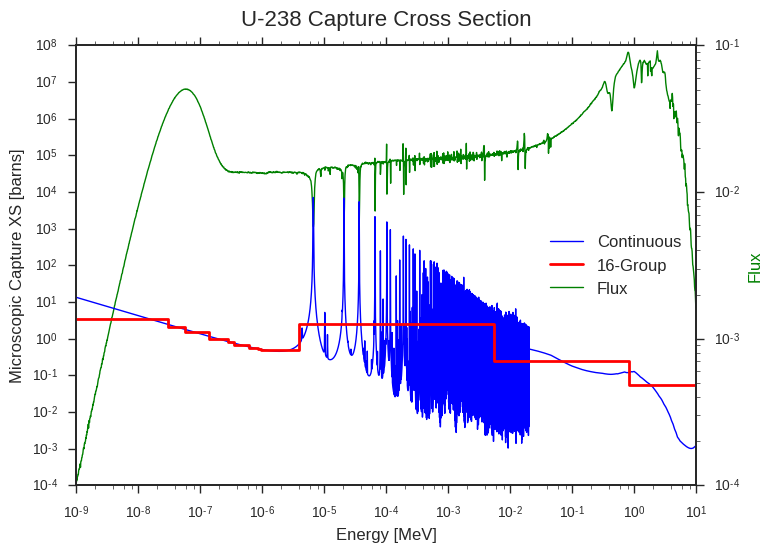
\includegraphics[width=0.9\linewidth]{figures/intro/u238-capture-16}
%  \caption{}
%\end{subfigure}
%\caption[Uranium-238 capture cross section]{Continuous energy and multi-group cross sections for U-238 capture in a PWR spectrum for 70-groups (a) and 16-groups (b).}
%\label{fig:pwr-ce-mg-xs}
%\end{figure}

